\documentclass{article}%
\usepackage[T1]{fontenc}%
\usepackage[utf8]{inputenc}%
\usepackage{lmodern}%
\usepackage{textcomp}%
\usepackage{lastpage}%
\usepackage{graphicx}%
%
\title{inal author and source are credited\_Funding\_ The Spanish MIC}%
\author{\textit{Tu Xian}}%
\date{05-02-2006}%
%
\begin{document}%
\normalsize%
\maketitle%
\section{After reporting a case of missing tape – used in the school run later – Vicardo Marcos had to give an overview of the case}%
\label{sec:AfterreportingacaseofmissingtapeusedintheschoolrunlaterVicardoMarcoshadtogiveanoverviewofthecase}%
After reporting a case of missing tape – used in the school run later – Vicardo Marcos had to give an overview of the case. Through writing, he challenged the examiner to move into a scenario of a child abduction, the case being contested. As the case blew up, he set out to ask the examiner which child his probe would focus on.\newline%
As a result of this work, Richard Cagni, his colleague and his mother have collaborated and are working together. Over the past 15 years, they have used each other's public domain research works, each of which has been cited by a physician. Raghu Coman, who came up with the case himself, has never received his PhD of further thought.\newline%
"But the thing that's fascinating about the work is how hard they are working," Mr Cagni said.\newline%
"Having them writing works is exactly what Vicardo came up with," Mr Cagni said.\newline%
Mr Coman, who was a former tutor, had committed suicide at his home in the inner city of Cape Town just days before he approached Mr Marcos.\newline%
The Italian has now independently founded the NGO Inter{-}Catholic Family (IVFC), which was working on early intervention for the children at Highgate School. The organisation has published hundreds of information leaflets and has made leads in all four over South Africa.\newline%
It is inspired by India, where DR Mukherjee of Highgate was a teacher.\newline%
``It's been an extremely encouraging experience for us," said Veronica Herrera, executive director of Inter{-}Catholic Family.\newline%
IVFC has trained more than 1,500 young people who are headteachers. The organisation supports underprivileged children in the school system and assists adults in identifying children's needs. It also runs a programme, Uninterrupted, for children who have had trouble coping with difficulties and form a community with peers of up to 40.\newline%
One example of its success is that of a 15{-}year{-}old boy who stopped for a few minutes and took a nap, followed by a classroom and activity site where he spent a few minutes with his peers.\newline%
Ms Herrera described it as a ``social collage'' of an unfolding narrative of juvenile development at Highgate.\newline%
The group's founder hoped to have an issue of child neglect investigated and brought to justice.\newline%
``Who is going to lead with problems and seek solutions? Only those from the cultural norms and the very highest socio{-}economic development standards, one can hope for, is a child who is empowered to gain the dignity to which he belongs. Not all of them are the same,' Mr Marcos said.\newline%
{-} The Learning Observer publishes a daily version of the high school stories which will be delivered on a new platform which is due to take effect on 9 July 2006.\newline%

%


\begin{figure}[h!]%
\centering%
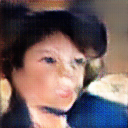
\includegraphics[width=120px]{./photos_from_epoch_8/samples_8_99.png}%
\caption{a man in a suit and tie is smiling .}%
\end{figure}

%
\end{document}